% =============================================================================

\vspace*{\fill}

\begin{figure}[!h]
\begin{lstlisting}[language=pseudo,style=block]
saes.v5.esrsub.lo rd, rs1, rs2 : rd = v5.SrSub(rs1, rs2, fwd=1, hi=0)
saes.v5.esrsub.hi rd, rs1, rs2 : rd = v5.SrSub(rs1, rs2, fwd=1, hi=1)
saes.v5.dsrsub.lo rd, rs1, rs2 : rd = v5.SrSub(rs1, rs2, fwd=0, hi=0)
saes.v5.dsrsub.hi rd, rs1, rs2 : rd = v5.SrSub(rs1, rs2, fwd=0, hi=1)
saes.v5.emix      rd, rs1, rs2 : rd = v5.Mix(rs1, rs2, fwd=1)
saes.v5.dmix      rd, rs1, rs2 : rd = v5.Mix(rs1, rs2, fwd=0)
saes.v5.sub       rd, rs1      : rd = SubBytes(rs1.8[i])         for i=0..3
\end{lstlisting}
\caption{
  Instruction mnemonics, and their mapping onto pseudo-code functions, for \ISE{5}.
}
\label{fig:v5:mnemonics}
\end{figure}

\begin{figure}[!h]
\begin{lstlisting}[language=pseudo,style=block]
v5.SrSub(rd, rs1, rs2, fwd, hi):
  if(fwd):
    if hi: tmp.32 = {rs1.8[3], rs2.8[0], rs2.8[1], rs2.8[2]}
    else : tmp.32 = {rs2.8[3], rs1.8[1], rs1.8[0], rs1.8[2]}
    tmp.8[i]      =    AESSBox[tmp.8[i]] for i=0..3
  else:
    if hi: tmp.32 = {rs2.8[3], rs2.8[0], rs1.8[1], rs2.8[2]}
    else : tmp.32 = {rs1.8[3], rs2.8[1], rs1.8[0], rs1.8[2]}
    tmp.8[i]      = InvAESSBox[tmp.8[i]] for i=0..3
  if(hi): rd.32 = {tmp.8[2],tmp.8[3],tmp.8[0],tmp.8[1]}
  else  : rd.32 = {tmp.8[1],tmp.8[3],tmp.8[0],tmp.8[2]}

v5.mix(rd, rs1, rs2, fwd):
  col0.32 = {rs1.8[2], rs1.8[3], rs2.8[2], rs2.8[3]}
  col1.32 = {rs1.8[0], rs1.8[1], rs2.8[0], rs2.8[1]}
  n0.8    = AESMixColumn(       col0   ) if fwd else AESInvMixColumn(       col0   )
  n1.8    = AESMixColumn(ROTL32(col0,8)) if fwd else AESInvMixColumn(ROTL32(col0,8))
  n2.8    = AESMixColumn(       col1   ) if fwd else AESInvMixColumn(       col1   )
  n3.8    = AESMixColumn(ROTL32(col1,8)) if fwd else AESInvMixColumn(ROTL32(col1,8))
  rd.32 = {n2, n3, n0, n1}
\end{lstlisting}
\caption{
  Instruction pseudo-code functions for \ISE{5}.
}
\label{fig:v5:pseudo}
\end{figure}

\begin{figure}[!h]
\begin{lstlisting}[language=pseudo,style=block]
lw                a0,  0(a4)   // Load Round Key
lw                a1,  4(a4)
lw                a2,  8(a4)
lw                a3, 12(a4)
xor               t0, t0, a0   // Add Round Key
xor               t1, t1, a1
xor               t2, t2, a2
xor               t3, t3, a3
saes.v5.esrsub.lo a0, t0, t1   // Quad 0: SubBytes / ShiftRows
saes.v5.esrsub.lo a1, t1, t0   // Quad 1
saes.v5.esrsub.hi a2, t2, t3   // Quad 2
saes.v5.esrsub.hi a3, t3, t2   // Quad 3
saes.v5.emix      t0, a0, a2   // Quad 0: ShiftRows / MixColumns
saes.v5.emix      t1, a1, a3   // Quad 1
saes.v5.emix      t2, a2, a0   // Quad 2
saes.v5.emix      t3, a3, a1   // Quad 3
\end{lstlisting}
\caption{
  An AES encryption round implemented using \ISE{5}.
}
\label{fig:v5:round}
\end{figure}

\vspace*{\fill}

% -----------------------------------------------------------------------------

\newpage

\vspace*{\fill}

\begin{figure}[!h]
\centering
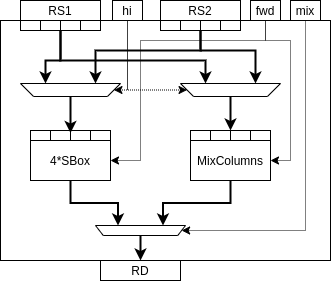
\includegraphics[width={0.5\textwidth}]{diagrams/ise-datapath-v5.png}
\caption{
  A diagrammatic description of the functional unit required to support \ISE{5}.
}
\label{fig:v5:fu}
\end{figure}

\vspace*{\fill}

% =============================================================================
